% results: space
% for brevity: report exact number!!!
% add new results on SenseGram

\documentclass[11pt]{article}
\usepackage{konvens2016}

\usepackage{times}
\usepackage{latexsym}
\usepackage{booktabs}
\usepackage{url}
\usepackage{graphicx}
\usepackage{acronym}
\usepackage[lined, ruled]{algorithm2e}
\usepackage[normalem]{ulem}
\usepackage{commath}
\usepackage{amsmath}
\makeatletter
\g@addto@macro\normalsize{%
  \setlength\abovedisplayskip{5pt}
  \setlength\belowdisplayskip{5pt}
  \setlength\abovedisplayshortskip{5pt}
  \setlength\belowdisplayshortskip{5pt}
}
\makeatother



\useunder{\uline}{\ul}{}

\newcommand{\gc}{\cellcolor[gray]{0.9}}
\newcommand{\parm}{ \mathord{\bullet}}
\urldef\myurl\url{https://www.cs.york.ac.uk/semeval-2013/task13/index.php%3Fid=results.html}


\usepackage{mathptmx}
\usepackage[scaled=.90]{helvet}
\usepackage{courier}

\usepackage{url}
\usepackage{latexsym}

%\setlength\titlebox{5cm}

% You can expand the titlebox if you need extra space
% to show all the authors. Please do not make the titlebox
% smaller than 5cm (the original size); we will check this
% in the camera-ready version and ask you to change it back.


\DeclareMathOperator*{\argmax}{arg\,max}

\newenvironment{description2}
    {\begin{description}
        \vspace{-0.2em}
        \setlength{\abovedisplayskip}{0pt}
        \setlength{\belowdisplayskip}{0pt}
        \setlength{\itemsep}{5pt}
        \setlength{\parskip}{0pt}
        \setlength{\parsep}{0pt}
        \setlength{\topsep}{0pt}
        \setlength{\partopsep}{0pt}
    }
    {\vspace{-0.2em}
    \end{description}}
%}


\newenvironment{itemize2}
    {\begin{itemize}
        \vspace{-0.2em}
        \setlength{\abovedisplayskip}{0pt}
        \setlength{\belowdisplayskip}{0pt}
        \setlength{\itemsep}{5pt}
        \setlength{\parskip}{0pt}
        \setlength{\parsep}{0pt}
        \setlength{\topsep}{0pt}
        \setlength{\partopsep}{0pt}
    }
    {\vspace{-0.2em}
    \end{itemize}}
%}


\newenvironment{enumerate2}
    {\begin{enumerate}
        \vspace{-0.1em}
        \setlength{\abovedisplayskip}{0pt}
        \setlength{\belowdisplayskip}{0pt}
        \setlength{\itemsep}{5pt}
        \setlength{\parskip}{0pt}
        \setlength{\parsep}{0pt}
        \setlength{\topsep}{0pt}
        \setlength{\partopsep}{0pt}
    }
    {\vspace{-0.1em}
    \end{enumerate}}
%}




\title{Noun Sense Induction and Disambiguation using \\ Graph-Based Distributional Semantics}

\author{Alexander Panchenko, Johannes Simon, Martin Riedl and Chris Biemann \\
  Technische Universit{\"a}t Darmstadt, Computer Science Department, LT Group  \\
  Hochschulstr. 10, Darmstadt, Germany \\
  {\tt \{panchenko,simon,riedl,biem\}@lt.informatik.tu-darmstadt.de}
  }

\date{}

\begin{document}
\maketitle
\begin{abstract}
We introduce an approach to word sense induction and disambiguation. The method is unsupervised and knowledge-free: sense representations are learned from distributional evidence and subsequently used to disambiguate word instances in context. These sense representations are obtained by clustering dependency-based second-order similarity networks. We then add features for disambiguation from heterogeneous sources such as window-based and sentence-wide co-occurrences, and explore various schemes to combine these context clues. Our method reaches a performance comparable to the state-of-the-art unsupervised word sense disambiguation systems including top participants of the SemEval 2013 word sense induction task and two more recent state-of-the-art neural word sense induction systems. 


\end{abstract}


\section{Introduction}
A word sense disambiguation (WSD) system takes as input a word and its context and outputs a sense of this word~\cite{Navigli2009}. While the goal of all such methods is the same, there are substantial differences in their implementation. Some systems use knowledge-based approaches that rely on handcrafted sense inventories, such as WordNet~\cite{miller1995wordnet}, while others use supervised approaches that learn from hand-labeled training data, such as SemCor~\cite{Miller1993}. However, hand-crafted lexical resources and training data are expensive to create, often inconsistent and domain-dependent. Furthermore, these methods assume a fixed sense inventory for each word. This is problematic as (1) senses emerge and disappear over time; (2)  different applications require different granularities of a sense inventory.

An alternative route explored in this paper is based on an unsupervised knowledge-free approach. Our method learns an interpretable sense inventory by clustering semantically similar words. To learn sense inventories, we rely on the JoBimText framework and distributional semantics~\cite{Biemann2013}, adding a word sense disambiguation functionality on top of it.

The key contribution of this paper is a framework that relies on such induced inventories as a pivot for learning contextual feature representations and uses them for disambiguation. The advantage of our method, compared to prior art, is that it can incorporate several types of context features in an unsupervised way. We demonstrate our approach, by combining four heterogeneous types of context features. The method achieves state-of-the-art results in unsupervised WSD.  
	


\section{Related Work}
\label{sec:relatedwork}

Approaches to WSD vary according to the level of supervision and according to the amount of external knowledge they use \cite{agirre2007word,Navigli2009}.  

\textit{Supervised approaches} use an explicitly sense-labeled training corpus to construct a model, usually building one model per target word. Successful machine learning setups include SVMs~\cite{Lee2002} and classifier ensembles \cite{Klein2002}. \newcite{Wee2010} shows that decision trees using bag-of-word features are unable to outperform the  most frequent sense baseline. 
Supervised approaches achieve the top performance in shared tasks on WSD such as SemEval, but require considerable amounts of sense-labeled examples. 

A WSD method that uses predefined dictionaries, lexical resources or semantic ontologies can be considered \emph{knowledge-based}. Knowledge-based systems rely on a lexical resource and vary from the classical \newcite{Lesk1986} algorithm that use word definitions to the \textit{BabelFy} \cite{moro2014entity} system that harnesses a multilingual semi-automatically constructed lexical semantic network. Knowledge-based approaches to WSD do not learn a model per target, but rather utilize information from a lexical resource that provides the sense inventory as well. Examples include \cite{Lesk1986,banerjee2002adapted,pedersen2005maximizing}.  %\newcite{moro2014entity} describe a system that harnesses a multilingual semi-automatically constructed lexical semantic network. % \newcite{miller2012using} describe a knowledge-based system that is able to exceed over the most frequent sense baseline for coarse-grained WSD, using word expansions from distributional similarity.

%Several experiments tested ``non-deep'' neural networks  for {WSD}, e.g.~\cite{Leacock1993,Mooney1996,Towell1998}. Later SVMs have been recognised as the most successful mechanism for supervised WSD~ \cite{Lee2002}. While Na\"ive Bayes classifiers are outperformed by more powerful methods such as SVMs, they generally compare well despite their independence assumption~\cite{Mooney1996,Ng1997,Leacock1998,Pedersen1998}. Instance-based models, also known as memory-based models, have also been found to be among the highest-performing methods on this task~\cite{Ng1997a,Daelemans1998}. Furthermore, ensembles of several supervised WSD systems surpass performance of each of the individual classifiers \cite{Klein2002,Florian2002}. 

%While supervised knowledge-rich approaches demonstrate top performance in competitions~\cite{}, these evaluation are commonly conducted on small vocabularies of frequent words. Supervised approaches suffer from the knowledge acquisition bottleneck. They assume that a tremendous amount of background knowledge (i.e., sense inventories or sense-labeled corpora) is readily available, which is only the case for popular languages, such as English, and only for very few domains.

In this paper we deal with \textit{unsupervised} and \textit{knowledge-free} WSD approaches. They use neither handcrafted lexical resources nor hand-annotated sense-labeled corpora. Instead, they induce word sense inventories automatically from corpora. According to \newcite{Navigli2009}, unsupervised WSD methods fall into two categories: context clustering \cite{pedersen1997distinguishing,Schutze1998} and word (ego-network) clustering~\cite{lin1998information,pantel2002,Widdows2002,Biemann2006,Hope2013}. 

\textit{Context clustering} methods, e.g.~\cite{Schutze1998}, represent an instance by a vector that characterizes its context, where the definition of context can vary greatly. These vectors of each instance are then clustered. 
%For instance, Sch\"utze \cite{Schutze1998}  represents contexts in an SVD-reduced bag-of-words vector space. Word sense clusters are then computed with the $k$-means algorithm. Later, Pantel and Lin~\shortcite{pantel2002discovering} used a two-staged \textit{Clustering by Committee} algorithm. In a first stage, it uses average-link clustering to find small and tight clusters. These are then input to the second stage, which iteratively identifies committees from these clusters. 
%In a manual evaluation, Pantel and Lin found their method to outperform $k$-means and average-link clustering. 
Sense embeddings methods extend word embeddings~\cite{mikolov2013efficient} so that they learn one embedding per word sense and are commonly fitted with a disambiguation mechanism \cite{Huang2012,tianEtAl2014,neelakantanefficient,bartunov2015breaking,li2015multi}. The approach of Pelevina et al.~\shortcite{pelevina2016} is similar to the one presented in this paper, but instead of sparse features the authors use word embeddings. 

The \emph{AI-KU} system \cite{Baskaya2013} is also based on context clustering. First, for each instance the system identifies the 100 most probable lexical substitutes using an $n$-gram model~\cite{Yuret2012}. Each instance is thus represented by a bag of substitutes. These vectors are clustered using $k$-means. The \emph{Unimelb} system by Lau et al.~\shortcite{Lau2013} implements context clustering using the Hierarchical Dirichlet Process (HDP) \cite{Teh2006}. Latent topics discovered in the training instances, specific to every word, are interpreted as word senses.  

Another class of word sense induction systems cluster \textit{word ego-networks}, rather than single instances of words. An ego network consists of a single node (ego) together with the nodes they are connected to (alters) and all the edges among those alters, cf. Figure \ref{graph-clustering-example}.  Nodes of an ego-network can  be (1) words semantically similar to the target word, as in our approach, or (2) context words relevant to the target, as in the \textit{UoS} system ~\cite{Hope2013}. Edges usually represent semantic similarities resp. association strength between nodes. The sense induction process using word graphs was previously explored by  \cite{Widdows2002,Biemann2010,Hope2013}. Disambiguation of instances is performed by assigning the sense with the highest overlap between the instance's context words and the words of the sense cluster, similar to the simplified Lesk algorithm.
% Ego-network clustering enables a more scalable solution to WSI since not all contests of a target in a very large corpus have to be pairwisely compared. 


%V\'{e}ronis~\shortcite{Veronis2004}  compiled a corpus for 10 polysemous nouns using a search engine. A word graph was built by drawing edges between co-occurring words within these word corpora. Edges below certain similarity threshold were discarded. Hubs of the network were interpreted as word senses. Disambiguation is this experiment was performed by computing the distance between context words and hubs in this graph. %No comparison to standardized evaluation  were performed. 

The \emph{UoS} system by Hope and Keller~\shortcite{Hope2013} builds a word ego-network with nodes being the 300 highest-ranked words in a dependency relation with the target word and clusters the graph to obtain senses weighted by word similarities. The graph is clustered with the MaxMax algorithm. Similar clusters are merged. Disambiguation of instances is performed by assigning the sense with the highest overlap between the instance's context words and the words of the sense cluster. 

While arguably the \emph{UoS} system is the most similar to ours, there are  crucial  differences. First, nodes in their ego network are (first-order) context features, not (second-order) similar words. Second, edge weights in our network represent the number of shared features, not the significance of co-occurrences. Finally, their disambiguation component relies on overlap between context and a sense's cluster words. 


Our system combines several of the above ideas, such as word sense induction based on clustering word similarities~\cite{pantel2002}, but in contrast to other unsupervised knowledge-free systems, we are able to combine and systematically evaluate the evidence from several features that model context differently.

\section{Data-Driven Noun Sense Modelling}

Our method consists of the three steps: computation of a distributional thesaurus, word sense induction, and building a disambiguation model of the induced senses. %The method is data-driven as it requires only a text corpus as input. It learns an interpretable disambiguation model, in contrast to word instance clustering WSI methods.  

\subsection{Distributional Thesaurus of Nouns}
\label{sec:dt-computation}

The goal of this step is to build a graph of word similarities, such as ``(tablet, notebook, 0.781)''.\footnote{We use the terms ``semantic similarity/relatedness'' to denote  scores derived with a distributional semantics approach. } To compute the graph, we used the \emph{JoBimText} framework \cite{Biemann2013}. While multiple alternatives exist  for computing of semantic similarity e.g.~\cite{mikolov2013efficient}, this framework is convenient in our case due to efficient computation of nearest neighbours for all words in the corpus while providing comparable precision~\cite{riedl2016phd}. For each noun in the corpus we retain the 200 most similar nouns. 
%Besides, we observed that related words yielded by this approach are more diverse than those of word embeddings, which is important for the word sense induction algorithm used in our method. 


%First, distributional features are extracted on a per-word basis from a text corpus. We rely on dependency-based features, such as {\small \textsf{amod($\parm$, grilled)}} or {\small \textsf{prep\_for($\parm$, dinner)}}, extracted with the Malt parser~\cite{nivre2007maltparser}, that are subsequently collapsed in the same way as the Stanford dependencies\footnote{\url{http://nlp.stanford.edu/software/stanford-dependencies.shtml}}. According to prior evaluations~\cite{panchenko2012study,Biemann2013} this kind of features provides state-of-the-art semantic similarity results. 

%Second, frequencies of words $f_{i*}$, features $f_{*j}$ and word-feature co-occurrences $f_{ij}$ are counted. Words, features and word-feature co-occurrences below a frequency of $t_w$, $t_f$ and $t_{wf}$, resp., are discarded. Based on these frequencies, significance scores for every word-feature co-occurrence are computed using the Local Mutual Information (LMI)~\cite{Evert2005}: $LMI(i, j) = f_{ij} \cdot PMI(i, j) = f_{ij} \cdot \log \frac{f_{ij} \sum_{i,j} f_{ij} }{f_{i*} \cdot f_{*j}}$. PMI is known to have a strong bias towards scoring low-frequency items. LMI mitigates the bias by multiplying the score by an co-occurrence frequency. By ranking features using this significance score, only the $p$ most significant features are chosen for every word.  In out experiments, word-feature frequencies below $t_{wf} = 2$ were dropped; each word was represented with  $p=1000$  features.
 
 
\begin{figure}
\begin{center}
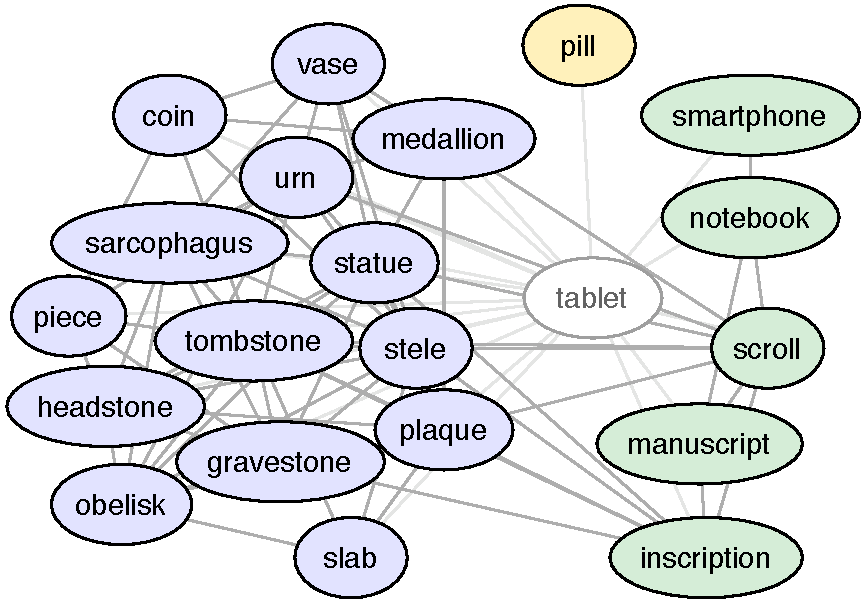
\includegraphics[width=0.45\textwidth]{figures/graph-clustering-new}
\end{center}
\caption{Visualization of the ego-network of the word ``tablet"  with three color-coded senses: ``stone'',  ``device'', and ``pill''. Note that the ego word ``tablet" is excluded from clustering.}
\label{graph-clustering-example}
\end{figure}
 
 % Using these features, word similarities are computed as a number of common features for two words: $sim(t_i, t_j) = | k: f_{ik} > 0 \wedge f_{jk} > 0 |$. This is again followed by a pruning step in which only the $l$ most similar terms are kept for every word. The pruning reduces computational complexity and noise.   
  


\subsection{Noun Sense Induction}

Similar to~\cite{pantel2002} and~\cite{Biemann2006}, we induce a sense inventory which represents senses with word clusters. For instance, the the sense ``tablet (device)" can be represented by the cluster ``smartphone, notebook, scroll, manuscript, inscription", see Figure~\ref{graph-clustering-example}. To compute the clustering, first we construct an ego-network $G$ of a word $t$ and then perform graph clustering of this network. An ego-network~\cite{everett2005ego_ALT} contains all nodes connected to the target node, called ``ego''. The identified clusters are interpreted as senses. Figure~\ref{graph-clustering-example} depicts an ego-network of ``tablet". Panchenko et al.~\shortcite{panchenko2013serelex} proposed a system for dynamic visualization of word ego-networks similar to those used in our method.\footnote{\url{http://www.serelex.org}} The key property of word ego-networks is that the words with similar senses tend to be connected, while having fewer connections to words from other senses, therefore forming clusters. 

%The method stems from approach of \newcite{Biemann2006}. 
The sense induction 
%presented in Algorithm~\ref{wsi-algo-pseudocode}. It
processes one word $t$ of the distributional thesaurus $T$ per iteration. First, we retrieve nodes of the ego-network $G$ being the $N$ most similar words $V$ of $t$ according to $T$. Note that the target word $t$ itself is not part of the ego-network. Second, we connect the nodes in $G$ to their $n$ most similar words from $T$. %To be more specific, we first retrieve $N$ most similar terms of each $v \in V$. Of these, only the top $n$ similar words are kept, each in $V$. 
Finally, the ego-network is clustered with the Chinese Whispers algorithm~\cite{Biemann2006}.
%, a time-linear variation of the Markov Chain Clustering~\cite{VanDongen2000}. We use this algorithm as they showed promising sense induction results in the past~\cite{Biemann2006}.  

The sense induction algorithm has two meta-parameters: the \emph{ego-network size} ($N$) of a target ego word $t$; and the \emph{ego-network connectivity} ($n$) each neighbour $v$ is allowed to have within the network. The parameter $n$ regulates the granularity of the inventory. In our experiments we set $N$ and $n$ to 200 to obtain a coarse-grained inventory. In preliminary experiments, we found inventories based on dependency features superior to other inventories, which is why we use only dependency-based similarities in our WSI experiments. 
%The $n$ is the upper bound of $N$. 
%In the ideal case, each sense of the target word, represented by the similar words belonging to the sense, forms a highly connected cluster that shows only few connections to other clusters (i.e.\ senses). %In our experiments, we have computed sense inventories based on distributional thesaurus $T$ computed with dependency features, as these provide the best results in lexical similarities according to previous studies~\cite{van2010mining,panchenko2013similarity}. 

\iffalse %comment start
\IncMargin{-1em}
\begin{algorithm}
\SetKwInOut{Input}{input}\SetKwInOut{Output}{output}

\Input{
$T$, distributional thesaurus, $N$,  ego-network size, $n$, ego-network connectivity }
\Output{for each term $w_k \in  T$, a clustering $S$ of its $N$ most similar terms}
\ForEach{$w_k \in  T$}{	
	$V \leftarrow$ $N$ most similar terms of $w_k$ according to $T$ \\
	$G \leftarrow$ graph with $V$ as nodes and no edges
	\BlankLine
	\ForEach{$v \in V$}{
		$V' \leftarrow$ $N$ most similar terms of $v$ according to $T$ \\
		\textbf{if} $v' \in V$ \textbf{then} add edge $(v, v')$ to $G$ for up to $n$ most similar terms 
	}
	$S \leftarrow$ \texttt{ChineseWhispers}($G$)\\
}
\caption{Word sense induction.}
\label{wsi-algo-pseudocode}

\end{algorithm}
\fi % comment end



\subsection{Disambiguation of Induced Noun Senses}

The goal of this step is to construct a disambiguation model  $P(s_i|C)$ for each of the induced senses $s_i \in S$, where $C$ is a feature representation of the target word $w$ in a context. We approximate the conditional probability of the sense $s_i$ in the context $C= \{ c_1,..., c_{m}\}$ with the Na\"ive Bayes model:  
\begin{equation}
P(s_i|C) = \frac{P(s_i)\prod_{j=1}^{|C|} P(c_j|s_i)}{P(c_1,...,c_m)},
\end{equation}
where the best sense given $C$ is chosen as following: $s_i^* = \argmax_{s_i} P(s_i)\prod_{j=1}^{|C|} P(c_j|s_i).$ To learn this model we use the assumption that words from a sense cluster $S$ are, to some extent, semantically substitutable. For example, consider the sense cluster that represents the ``fish'' sense of the word ``bass'': \{trout, catfish, eel, perch\} and the following sentence: ``\textit{Most fish such as $\parm$ live in freshwater lakes and rivers}''. As can be observed in this example, similar words usually occur in similar contexts and thus often have similar context features. As it will be clear from our experiments, in spite of inherent noise in such training data one can use these data for training a disambiguation model. 

Based on this assumption, it is possible to extract sense representations by aggregation of features from all words of the cluster $s_i$: we simply count in the training corpus the number of co-occurrences $f(w_k,c_j)$ and the cluster word $w_{ik}$ with the context feature $c_j$ across all words belonging to the sense cluster $s_i$: $\{w_1,...,w_n\}$. 
 
We cannot directly count any sense frequencies $f(s_i)$ or joint sense-feature frequencies $f(s_i, c_j)$ from an unlabeled text corpus. To estimate these frequencies we utilize an implication of our hypothesis: since two similar words are assumed to be substitutable, we assume any occurrence of the $i$-th  word from the $k$-th cluster, denoted as $w_k$, to be interchangeable with an occurrence of sense $s_i$. The frequency of ${s_i}$ is then given by $f({s_i}) = \sum_i^{|s_i|}f(w_k)$, where $|s_i|$ is the number of words in the sense cluster $s_i$. The same principle can be applied to determine a joint frequency $f({s_i}, c_j)$. To estimate the probability of a sense feature given a cluster word, we normalize the joint frequency by word frequency. This solves the problem of dominating high frequency cluster words:
\begin{equation}
P(c_j|w_k) = \frac{\displaystyle f(w_k,c_j)}{\displaystyle f(w_k)}.
\end{equation}
 

A sense cluster usually contains a large number of similar words (up to $N = 200$ in our case). Often there is a high discrepancy among the similarities of the cluster words to the target word. Thus, some words better represent the sense than the others. To account for this effect, we introduce an additional weighting coefficient $\lambda_k$ that is equal to the similarity between $k$-th cluster word $w_k$ and the target word $w$ being disambiguated. 

While cluster words may be ambiguous, this issue is compensated by the fact that most cluster words have common features, while the  noisy features of ambiguous words are specific to these words: they are not confirmed by noisy features of other ambiguous words. In some cases this assumption does not hold, e.g. the word ``Chelsea'' is similar to other words such as ``Milan'' or ``Barcelona'' that can represent both either a club or a city.

To normalize the score we divide it by the sum of all the weights $\Lambda_i = \sum_k^{|s_i|} \lambda_k$:
\begin{equation}
P(c_j|{s_i}) = \frac{1-\alpha}{\Lambda_i} \sum_k^{|s_i|} \lambda_k \frac{\displaystyle f(w_k,c_j)}{\displaystyle f(w_k)}+ \alpha,
\end{equation}
where $\alpha$ is a small number, e.g. $10^{-5}$, added for smoothing. 

The prior probability of each sense is computed based on the largest cluster heuristic: 
\begin{equation}
P({s_i}) =  \frac{|s_i|}{\sum_{s_i \in S} |s_i|}.
\end{equation}
We also explored estimation of the prior by a weighted average of cluster word counts, but this method provided lower results: 
\begin{equation}
P({s_i}) = \frac{1}{\Lambda_i} \sum_k^{|s_i|} \lambda_k\ f(w_k).
\end{equation}

Note that to calculate the sense models we only need (1) the distributional thesaurus $T$; (2) sense clusters; and (3) word-feature frequencies: $f(w_k) = f_{n*}$, and $f(w_k,c_j) = f_{nm}$, where $n$ is the index of the word $w_k$ and $m$ is the index of the feature $c_j$ in a word-feature matrix. Finally, sense features are pruned: in our experiments, each sense $s_i$ is represented with its most significant 20,000 context features in terms of $P(c_j|s_i)$. 

\subsection{Feature Extraction and Combination}
Our method learns separate models $P(s_i|C)$ for each type of context features. During classification, we either use these single-featured models directly or combine them at the feature- or meta-levels as described below. 

\paragraph{Single features.} 

We use four groups of  word-feature counts $f(w_k,c_j)}$ listed below to estimate probability of the feature given a sense $\hat P(c_j|{s_i})$. A single-sense model is then trained for each of these feature types. Note that our framework allow using of any other context features if one can estimate $f(w_k,c_j)$ for it. 

\begin{itemize2}

\item \textbf{Cluster features} directly use words from the induced sense clusters, i.e. the $\hat{P}(c_j|s_i)$ is equal to the similarity score $\lambda_{kj}$ between the target word $w_k$ and the context word $c_j$. 

\item \textbf{Dependency features} of a target word $w_k$ are all syntactic dependencies attached to it. For instance, the word ``tablet" has features such as ``subj($\parm$,type)'' or ``amod(digital,$\parm$)'', where ``$\parm$'' represents the position of the target word. During disambiguation, we use this kind of features in two modes: the first one, denoted as \textit{Deptarget}, represents the context $C$ as a set of all dependencies attached to the target word being disambiguated; the second mode, denoted as \textit{Depall} represents the context $C$ with dependencies of all words in the sentence, not just the target word. This is an expansion of the feature representation aiming to compensate the sparsity of the dependency representation.


\item \textbf{Dependency word features}, denoted as \textit{Depword}, are extracted from all syntactic dependencies attached to a target word $w_k$. Namely, we reduce dependency features to dependent words. For instance, the feature ``subj($\parm$,write)'' would result in the feature ``write''. We also experimented with  word co-occurrences, but they  provided lower results.

\item \textbf{Trigram features} are pairs of left and right words around the target word $w_k$. For instance, the word ``tablet" has features such as ``typing\_$\parm$\_or'' and ``digital\_$\parm$\_.''. Similarly to the dependency features, we use two modes to build the context $C$: the \textit{Trigramtarget} represents the target word with one trigram extracted from its context; the \textit{Trigramall} represents the target word with trigrams extracted from all words in the sentence. 

\end{itemize2}

\paragraph{Feature-level combination of features. } This method builds the set of context features $C$ uniting different  context features under combination, such as dependencies and trigrams. Next, we use the Na\"ive Bayes model based on this extended context representation to estimate $\hat{P}(s_i|C)$, using conditional probabilities $\hat{P}(c_j|s_i)$ depending on the type of the corresponding feature $c_j \in C$. 

\paragraph{Meta-level combination of features.} This method starts by performing independent sense classifications with the combined models. Afterwards, these predictions are aggregated using one of the three following strategies:

\begin{itemize2}

\item \textbf{Majority} selects the sense $s_i$ selected by the largest number of single models. 
\item \textbf{Ranks}. First, results of single model classification are ranked by their confidence $\hat{P}(s_i|C)$: the most suitable sense to the context obtains rank one and so on. Finally, we assign the sense with the least sum of ranks.
\item \textbf{Sum}. This strategy assigns the sense with the largest sum of classification confidences i.e., $\sum_i\hat{P}(s_i|C^i_k)$, where $i$ is the number of the single model.  
\end{itemize2}



\begin{figure*}
\begin{center}
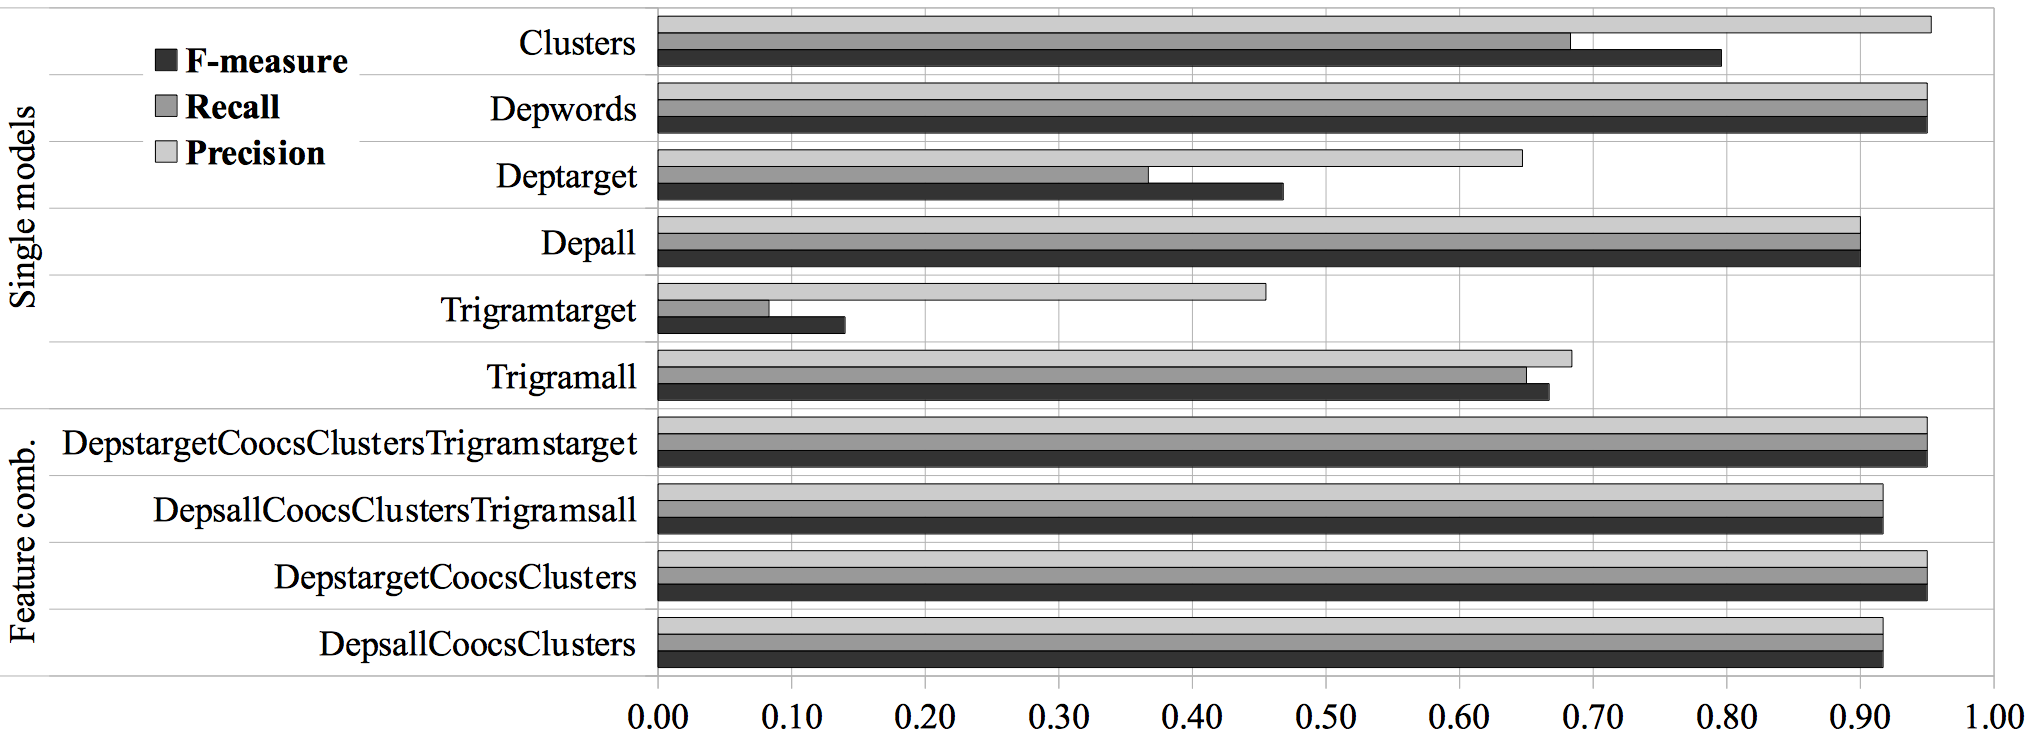
\includegraphics[width=0.92\textwidth]{figures/prj}
\end{center}
\caption{Performance of our method on the PRJ dataset. The models based on the meta-combinations are not shown for brevity as they did not improve performance of the presented models in terms of F-score. }
\label{tbl:results-prj}
\end{figure*}



%
%\begin{table*}
%\centering
%\scriptsize
%\begin{tabular}{llrrr}
%\toprule
%
%\bf Model & & \bf Precision & \bf Recall & \bf F-score  \\
%\toprule
%
%Single models & Clusters & \bf 0.953 & 0.683 & 0.796 \\
% & Depwords & \bf 0.950 & 0.950 & \underline{\bf0.950} \\
% & Deptarget & 0.647 & 0.367 & 0.468 \\
% & Depall & 0.900 & 0.900 & 0.900 \\
% & Trigramtarget & 0.455 & 0.083 & 0.140 \\
% & Trigramall & 0.684 & 0.650 & 0.667 \\
%\midrule
%
%Feature comb. & DepstargetCoocsClustersTrigramstarget & 0.950 & 0.950 & \underline{\bf 0.950} \\
% & DepsallCoocsClustersTrigramsall & 0.917 & 0.917 & 0.917 \\
% & DepstargetCoocsClusters & 0.950 & 0.950 & \underline{\bf 0.950} \\
% & DepsallCoocsClusters & 0.917 & 0.917 & 0.917 \\
%
%\midrule
%
%Meta comb. & Clusters+Depstarget+Depwords+Trigramstarget: majority & 0.940 & 0.783 & 0.854 \\
% & Clusters+Depstarget+Depwords+Trigramstarget: ranks & 0.941 & 0.533 & 0.681 \\
% & Clusters+Depstarget+Depwords+Trigramstarget: sum & 0.943 & 0.833 & 0.885 \\
% & Clusters+Depsall+Depwords+Trigramsall: majority & 0.898 & 0.883 & 0.890 \\
% & Clusters+Depsall+Depwords+Trigramsall: ranks & 0.927 & 0.633 & 0.752 \\
% & Clusters+Depsall+Depwords+Trigramsall: sum & 0.917 & 0.917 & 0.917 \\
% & Clusters+Depstarget+Depwords: majority & 0.906 & 0.800 & 0.850 \\
% & Clusters+Depstarget+Depwords: ranks & 0.903 & 0.467 & 0.616 \\
% & Clusters+Depstarget+Depwords: sum & 0.943 & 0.833 & 0.885 \\
% & Clusters+Depsall+Depwords: majority & 0.933 & 0.933 & \bf 0.933 \\
% & Clusters+Depsall+Depwords: ranks & \underline{\bf 1.000} & 0.717 & 0.835 \\
% & Clusters+Depsall+Depwords: sum & 0.900 & 0.900 & 0.900 \\
%
%
%\bottomrule
%\end{tabular}
%
%\caption{Performance of our method on the PRJ dataset. Top values of Precision and F-measure of our approach are set in boldface; the best are underlined. }
%\label{tbl:results-prj}
%\end{table*}


\section{Results}

We evaluate our method on three complementary datasets: (1) a small-scale collection of homonyms used for convenient interpretation of results; (2) a large-scale collection of homonyms and polysemous senses used for development of meta-parameters; and (3) a  mid-scale SemEval dataset used for comparison with other systems.\footnote{The datasets and the evaluation scripts: \url{http://github.com/tudarmstadt-lt/context-eval}.} 

In the experiments described below, we trained models on two corpora commonly used for training distributional models: ukWaC~\cite{ferraresi2008introducing} and Wikipedia\footnote{We used a dump of Wikipedia of October 2015: \url{http://panchenko.me/data/joint/corpora/en59g/wikipedia.txt.gz}}. Table~\ref{tbl:corpora} presents statistics about these two text collections.

\begin{table}
\footnotesize
\centering
\begin{tabular}{lcccc}
  \toprule          
  &  \bf   \# Tokens & \bf  Size & \bf Text Type \\ \midrule          
  Wikipedia & 1.863 $\cdot$ $10^9$ & 11.79 Gb & encyclopaedic \\
  ukWaC & 1.980 $\cdot$ $10^9$ &  12.05 Gb & Web pages \\
  \bottomrule  
\end{tabular}
\caption{Corpora used for training our models.}
\label{tbl:corpora}
\end{table}
   

\subsection{Evaluation on PRJ }
The goal of this evaluation is to make sure the method performs as expected in case of homonyms. %We chose a small dataset to be able to track each misclassified context. 

\paragraph{Dataset.} 
This dataset consists of 60 contexts of the words ``python", ``ruby" and ``jaguar", hence the name of the dataset (PRJ). Each word has two homonymous senses, respectively ``snake" or ``programming language", ``gem" or ``programming language", and ``animal" or ``car", respectively. Contexts were randomly sampled from the first three paragraphs of the corresponding Wikipedia articles. Each sense is represented with 10 contexts. We manually assigned senses from the  induced inventory derived from the ukWaC corpus. We used the model trained on the ukWaC corpus. 

\paragraph{Evaluation metrics.} The contexts are labeled  with the induced senses, so we directly use precision and recall without mapping of inventories.  

\paragraph{Discussion of results.} Agirre and Soroa~\shortcite{agirre2007word} suggest that the WSD of homonyms is an almost solved problem for supervised systems, reaching F-scores above 0.90. Our results summarized in Table~\ref{tbl:results-prj} confirm this for the unsupervised approach. Our method reaches a precision up to 0.953  and an F-score of 0.950. 

The three misclassified samples by the system that reached an F-score of 0.950 are the following. The first one is from the article about ``ruby (gem)" which describes possible colors of ruby gems. It was wrongly labeled with the ``ruby (color)" sense. The second misclassified example from the ``jaguar (animal)" article contains multiple named entities, such as "USA" that strongly relate to economic activities such as car production. Finally, the reason of  misclassification of the third context from the ``python (snake)" article is that the ``molurus" feature received a high score in the ``language" sense. We attribute this learning error to the unbalanced nature of the ukWaC, as in the model trained on Wikipedia this feature has a higher score for the ``snake" sense. Thus, we conclude that our approach performs as expected in simple cases, yielding only few errors. 

Combinations of the single predictors neither provide extra improvement in these simple settings: none of the combined models improve the overall results, nor do they introduce any extra errors (see Figure~\ref{tbl:results-prj}). 


\subsection{Evaluation on TWSI}

The goal of this evaluation is to test performance of our method on a large scale dataset that contains both homonyms and polysemous senses. 

\paragraph{Dataset.} This test collection is based on a large-scale crowdsourced resource~\cite{Biemann2012} that comprises 1,012 frequent nouns with average polysemy of 2.33 senses per word. For these nouns, 145,140 annotated sentences are provided. Besides, a sense inventory is explicitly provided, where each sense is represented with a list of words that can substitute target noun in a given sentence. The sense distribution across sentences in the dataset is highly skewed resulting in 79\% of contexts assigned to the most frequent senses. 


\paragraph{Evaluation metrics.}
To compute performance we create an explicit mapping between the system-provided sense inventory and the TWSI  senses: senses are represented as bag of words vectors, which are compared using cosine similarity. Every induced sense gets assigned at most one TWSI sense. Once the mapping is completed, we can calculate precision and recall of the sense labeling with respect to the original TWSI labeling.

Note that performance of a disambiguation model depends on quality of the sense mapping. Therefore, we use five baselines that facilitate interpretation of the results: 
\begin{enumerate2}
\item \textbf{MFS of the TWSI inventory} assigns the most frequent sense in the TWSI dataset. 
\item \textbf{Random sense of the TWSI inventory}.
\item \textbf{MFS of the induced inventory} assigns the identifier of the largest sense cluster.
\item \textbf{Upper bound of the induced vocabulary} selects the correct sense for the context, but only if the mapping exist for this sense. %Therefore, a disambiguation system cannot perform better using a given sense inventory. %the difficulty of WSD given the test set; if there are few polysemous words, this baseline will converge towards the MFS baseline; with a large number of senses, this can be a lower baseline.
\item \textbf{Random sense of the induced inventory}. % selects a random sense. % the correct sense for the context, but only if the mapping exist for this sense. Therefore, a disambiguation system cannot perform better using a given sense inventory.
\end{enumerate2}



\paragraph{Discussion of results.}

Table~\ref{tab:results-twsi} presents evaluation of our method trained on the Wikipedia corpus  (comparison of these results with the ukWaC corpus is provided in Figure~\ref{fig:wiki-vs-ukwac}). 
First, one can observe that, similarly to the PRJ dataset, the \textit{Cluster} features yield a precise results up to $P=0.719$. Yet, recall of these feature is inherently limited by the size of these clusters (15 to 200 words as compared to up to 20,000 for other types of features). Besides, \textit{Trigramtarget} features yield even higher precision of 0.729, but their recall of 0.193 is even less than that of clusters. The single model based on the \textit{Deptarget} features balances precision and recall, reaching F-measure of 0.571 at $P=0.709$. 

Several models based on feature- and meta-level combinations clearly outperform single-feature models. The best scores in terms of F-score (0.696-0.698) are obtained by a combination of four feature types (\textit{Deptarget, Depword, Cluster, Trigramtarget}) at the feature level or using the sum meta-combination. Similar results (F-score of 0.694-0.695) can be obtained via combination of the same features without the \textit{Trigramtarget}. In terms of precision, the best results are delivered by a meta-combination  of the above-mentioned features, combined by summing their ranks. In these settings, the combined models yield precision of 0.713-0.720.

Figure~\ref{fig:wiki-vs-ukwac} compares the performance of our models trained on the Wikipedia corpus and the ukWaC corpus. The Wikipedia-based models consistently outperform their counterparts trained on the ukWaC. This can be attributed to the fact that the TWSI contexts were originally sampled from the Wikipedia. Besides, Wikipedia is a more balanced and ``clean" corpus than ukWaC. 

All our models outperform the random sense baselines and the most frequent sense (MFS) baseline of the induced inventory in terms of precision and most of them outperforms these baselines in terms of F-score. These results show that the features used in our technique indeed provide a strong signal for  word sense disambiguation. However, none of our models was able to outperform the most frequent sense of the TWSI. 

We assumed that this is  due to the highly skewed nature of the dataset where 79\% of contexts are associated with the most frequent sense. To validate the hypothesis that our system yields state-of-the-art performance in spite of this result we compared its performance to a recent unsupervised WSD system based on sense embeddings, called AdaGram~\cite{bartunov2015breaking}. This is a multi-prototype extension of the Skip-gram model~\cite{mikolov2013efficient}, which relies on Bayesian inference to perform sense disambiguation. We chosen this method as it yields state-of-the-art results, outperforming other approaches based on sense embeddings, such as~\cite{neelakantanefficient}. We tried several models varying the $\alpha$ parameter that controls granularity of the induced sense inventory. The best AdaGram configuration with the $\alpha=$ equals 0.05 yields F-score on of 0.656, which is below the most frequent sense of the TWSI, similarly to our model \textit{DeptargetDepwordClusterTrigramtarget} that reaches F-score of 0.698.  

\begin{table*}[t!]
\scriptsize

\centering
%\begin{tabular}{@{~}l@{}r|rr@{~~~}r|rr@{~~~}r@{~}}
%\toprule


\centering
\begin{tabular}{llrrrr}
\toprule

\bf Model & & \bf \#Senses & \bf Precision & \bf Recall & \bf F-score  \\
\toprule
TWSI baselines & MFS of the TWSI inventory   & 2.31  & 0.787 &	0.787&	0.787  \\
& Random sense of the TWSI inventory & 2.31 & 0.535 & 0.535 &	0.535  \\
\midrule
Induced baselines & Upper bound of the induced inventory  & 1.64    & 1.000  & 0.746 &  0.855 \\
& MFS of the induced inventory  & 1.64 & 0.642 & 0.642  & 0.642  \\
& Random Sense of the induced inventory  & 1.64 & 0.559 &	0.558	& 0.558   \\
\midrule
Sense embeddings & AdaGram, $\alpha = 0.05$, upper bound of induced inv. & 4.33 & 1.000 & 0.865 & 0.928 \\
& AdaGram, $\alpha = 0.05$ & 4.33 & 0.656 & 0.656 & 0.656 \\ 


\toprule

Single models & Cluster  & 1.64 & \bf 0.719 & 0.405 & 0.518  \\
& Depword & 1.64 & 0.684 & 0.684 & 0.684 \\
& Deptarget & 1.64 & 0.709 & 0.571 & 0.633 \\
& Depall & 1.64 & 0.689 & 0.689 & 0.689 \\
& Trigramtarget & 1.64 & \bf \underline{0.729} & 0.193 & 0.305 \\
& Trigramall & 1.64 & 0.670 & 0.561 & 0.611 \\
\midrule 
Feature comb. & DeptargetDepwordClusterTrigramtarget  & 1.64 &  0.698 & \bf \underline{0.698} & \bf \underline{0.698} \\
 & DepallDepwordClusterTrigramall  & 1.64 & 0.697 & \bf 0.697 & \bf 0.697 \\
 & DeptargetDepword Cluster  & 1.64 & 0.694 & \bf 0.694 & \bf 0.694 \\
 & DepallDepwordCluster  & 1.64 & 0.691 & \bf 0.691 & 0.691 \\
\midrule 
Meta comb. & Cluster+Deptarget+Depword+Trigramtarget: majority & 1.64 & \bf 0.718 & 0.605 & 0.656 \\
  & Cluster+Deptarget+Depword+Trigramtarget: ranks & 1.64 & 0.687 & 0.360 & 0.472 \\ 
  & Cluster+Deptarget+Depword+Trigramtarget: sum & 1.64 &  0.696 & \bf 0.696 & \bf 0.696 \\
  & Cluster+Depall+Depword+Trigramall: majority & 1.64 & 0.692 & 0.685 & 0.688 \\
  & Cluster+Depall+Depword+Trigramall: ranks & 1.64 & \bf 0.715 & 0.420 & 0.529 \\
  & Cluster+Depall+Depword+Trigramall: sum & 1.64 & 0.693 & 0.693 & 0.693 \\
  & Cluster+Deptarget+Depword: majority & 1.64 & 0.704 & 0.630 & 0.665 \\
  & Cluster+Deptarget+Depword: ranks & 1.64 & 0.713 & 0.410 & 0.521 \\
  & Cluster+Deptarget+Depword: sum & 1.64 & 0.695 & 0.695 & \bf 0.695 \\
  & Cluster+Depall+Depword: majority & 1.64 & 0.689 & 0.688 & 0.688 \\
  & Cluster+Depall+Depword: ranks & 1.64 & \bf 0.720 & 0.406 & 0.519 \\
  & Cluster+Depall+Depword: sum & 1.64 & 0.693 & 0.693 & 0.693 \\


\bottomrule
\end{tabular}
\caption{Performance of our method on the TWSI dataset trained on the Wikipedia corpus. Top 5 scores of our approach per section are set in boldface; the best scores are underlined.}
\label{tab:results-twsi}
\end{table*}


\begin{figure*}
\begin{center}
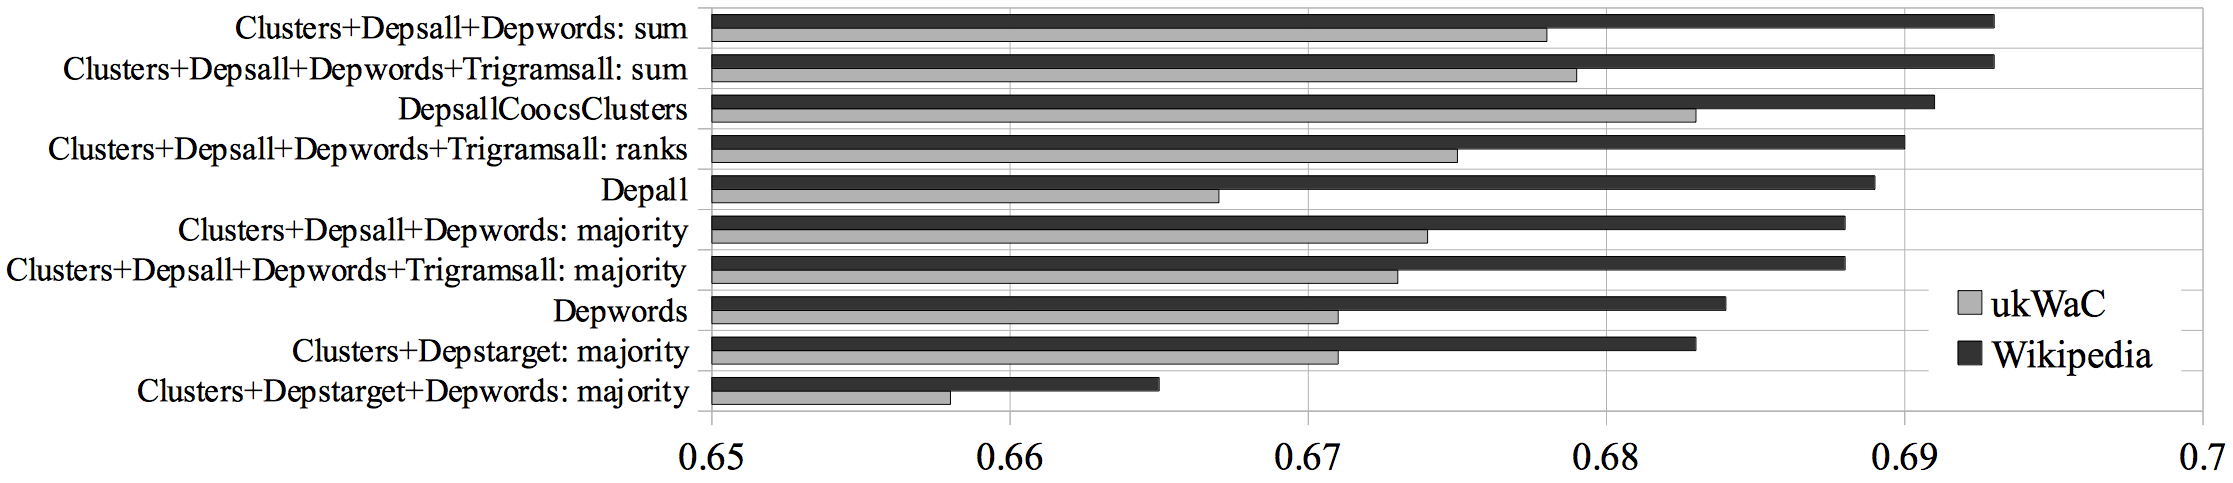
\includegraphics[width=1.0\textwidth]{figures/ukwac-wiki-4}
\end{center}
\caption{Effect of the corpus choice on the WSD performance: 10 best models according to the F-score on the TWSI dataset trained on Wikipedia and ukWaC corpora. }
\label{fig:wiki-vs-ukwac}
\end{figure*}

\subsection{Evaluation on SemEval-2013 Task 13}

The goal of this evaluation is to compare performance of our method to the state-of-the-art unsupervised WSD systems.


\paragraph{Dataset.}  


The SemEval-2013 task 13 ``Word Sense Induction for Graded and Non-Graded Senses"~\cite{Jurgens2013} provides 20 nouns, 20 verbs and 10 adjectives in WordNet-sense-tagged contexts. It contains 20-100 contexts per word, and 4,664 contexts in total, which were drawn from the Open American National Corpus. In our experiments, we use the 1,848 noun-based contexts. Participants were asked to cluster these 4,664 instances into groups, with each group corresponding to a distinct word sense. We report result on the 20 nouns as our method is designed for modelling of noun senses.

\paragraph{Evaluation metrics.}  Performance is measured with three measures  that require a mapping of sense inventories (Jaccard Index, Tau and WNDCG) and two cluster comparison measures (Fuzzy NMI and  Fuzzy B-Cubed).\footnote{Detailed interpretation of the five performance metrics: \myurl} During evaluation the test data is divided into five segments: four of which are used to build the mapping, and one for evaluation. 


% using the method of \newcite{jurgens2012evaluation}

% Goal of the  task is to detect instances with multiple senses and score each sense using a range between 0 and 1.  Performance of single sense assignments is quantified with \textit{F-measure}, \textit{NMI} and \textit{B-Cubed} metrics. For the graded sense assignments performance is measured with \textit{Jaccard Index}, \textit{WNDCG}, \textit{Fuzzy NMI}, and \textit{Fuzzy B-Cubed}. Note that (fuzzy) \textit{NMI} and \textit{B-Cubed} directly compare two clusterings while other metrics require a mapping of inventories. 

\paragraph{Discussion of results.}

Participating teams in this task were \emph{AI-KU}~\cite{Baskaya2013}, \emph{Unimelb}~\cite{Lau2013}, \emph{UoS}~\cite{Hope2013} and \emph{La Sapienza}. The latter relies on WordNet as sense inventory and uses a knowledge-rich approach to disambiguation. Only the \emph{UoS} used an induced sense inventory, similarly to us, while all other participating teams performed sense clustering directly on the disambiguation instances, thus not being able to classify additional instances without re-clustering the whole dataset.

Table~\ref{tab:results-semeval} compares the performance of our method to other approaches. As one may observe, most of the combined models only sightly improve over the single-feature models according to Jaccard Index and Fuzzy NMI. However, one class of combined models that achieves a consistent improvement over the single-feature systems is the meta-combination based on the sum of ranks. Similarly to the TWSI experiment, the two best combined models are based either on four (\textit{Deptarget, Depword, Cluster, Trigramtarget}) or three (\textit{Deptarget, Depword, Cluster}) features. These two models perform comparably to the best participants of the SemEval challenge or outperform them, depending on the metric. On one hand, the top SemEval system  (AI-KU remove5-add1000) reaches a Jaccard Index of 0.229 while our approach obtains scores of up to 0.219. The second best SemEval system according to this metric (UoS top-3) has a score of 0.220. On the other hand, according to the Tau and Fuzzy B-Cubed scores, our best systems outperform the SemEval participants.  Therefore, we conclude that performance of our approach is comparable to the other unsupervised state-of-the-art word sense disambiguation approaches.

Finally, note that none of the unsupervised WSD methods discussed in this paper, including the top-ranked SemEval submissions and the method based on sense embeddings (AdaGram~\cite{bartunov2015breaking} and SenseGram~\cite{pelevina2016}), were able to beat the most frequent sense baselines of the respective datasets. Similar results are observed for other recently proposed unsupervised word sense disambiguation methods~\cite{nietopina2016}.  

\begin{table*}[t]
\scriptsize

\centering
\begin{tabular}{llrrr|rr}
\toprule

 \bf Model &  & \bf Jacc. Ind. & \bf Tau & \bf WNDCG & \bf Fuzzy NMI & \bf Fuzzy B-Cubed \\
\toprule
Baselines & One sense for all & 0.171 & 0.627 & 0.302 & 0.000 & 0.631 \\
& One sense per instance & 0.000 & 0.953 & 0.000 & 0.072 & 0.000 \\
& Most Frequent Sense (MFS) & 0.579 & 0.583 & 0.431 &  -- & -- \\
\toprule

SemEval systems & AI-KU (add1000) & 0.176 & 0.609 & 0.205 & 0.033 & 0.317 \\
& AI-KU & 0.176 & 0.619 & 0.393 & \bf \underline{0.066} & 0.382 \\
& AI-KU (remove5-add1000) & \bf 0.228 & \bf 0.654 & 0.330 & 0.040 & 0.463 \\
& Unimelb (5p) & 0.198 & 0.623 & 0.374 & 0.056 & 0.475 \\
& Unimelb (50k) & 0.198 & 0.633 & 0.384 & 0.060 & \bf 0.494 \\
& UoS (\#WN senses) & 0.171 & 0.600 & 0.298 & 0.046 & 0.186 \\
& UoS (top-3) & 0.220 & 0.637 & 0.370 & 0.044 & 0.451 \\
& La Sapienza (1) & 0.131 & 0.544 & 0.332 & --  & -- \\
& La Sapienza (2) & 0.131 & 0.535 & \bf \underline{0.394} & -- & -- \\
\midrule
Sense embeddings & AdaGram, 100 dim., $\alpha$ = 0.05, & \bf \underline{0.274} & 0.644  & 0.318  & 0.058  & 0.470 \\
& SenseGram, 100 dim., w2v -- weighted -- sim. -- filter ($p=2$) & 0.197 & 0.615 & 0.291 & 0.011 & 0.615 \\
& SenseGram, 100 dim., JST  -- weighted -- sim. -- filter ($p=2$) & 0.205 & 0.624 & 0.291 & 0.017 & 0.598\\
\toprule

Single models & Cluster & 0.196 & 0.652 & 0.319 & 0.032 &  0.610 \\
 & Depword & 0.196 & 0.652 & 0.319 & 0.032 &  0.610 \\
 & Deptarget & 0.189 & 0.655 & 0.314 & 0.025 &  0.610 \\
 & Depall & 0.188 & 0.650 & 0.313 & 0.029 & 0.608 \\
 & Trigramtarget & 0.179 & 0.632 & 0.303 & 0.009 & \bf \underline{0.616} \\
 & Trigramall & 0.182 & 0.650 & 0.302 & 0.015 & 0.594 \\ 
\midrule
Feature comb. & DeptargetDepwordClusterTrigramtarget & 0.188 & 0.654 & 0.317 & 0.032 & \bf  0.611 \\
 & DepallDepwordClusterTrigramall & 0.197 & 0.652 & 0.317 & 0.034 & \bf 0.611 \\
 & DeptargetDepwordCluster & 0.189 & 0.655 & 0.318 & 0.033 & \bf  0.611 \\
 & DepallDepwordCluster & 0.197 & 0.651 & 0.317 & 0.034 & \bf 0.611 \\

\midrule

Meta comb. & Cluster+Deptarget+Depword+Trigramtarget: majority & 0.197 & 0.645 & 0.317 & 0.037 & 0.600 \\
 & Cluster+Deptarget+Depword+Trigramtarget: ranks & {\bf 0.219} & \bf 0.657 & 0.309 & 0.034 & 0.487 \\
 & Cluster+Deptarget+Depword+Trigramtarget: sum & 0.204 & 0.646 & 0.320 & 0.040 & 0.607 \\
 & Cluster+Depall+Depword+Trigramall: majority & 0.196 & 0.646 & 0.315 & 0.035 & 0.601 \\
 & Cluster+Depall+Depword+Trigramall: ranks & 0.216 & 0.654 & 0.316 & 0.042 & 0.526 \\
 & Cluster+Depall+Depword+Trigramall: sum & 0.193 & 0.651 & 0.317 & 0.034 & 0.605 \\
 & Cluster+Deptarget+Depword: majority & 0.200 & 0.647 & 0.317 & 0.039 & 0.601 \\
 & Cluster+Deptarget+Depword: ranks & \bf 0.217 &  \underline{\bf 0.659} & {\bf 0.324} & {\bf 0.048} & 0.533 \\
 & Cluster+Deptarget+Depword: sum & 0.204 & 0.647 & 0.319 & 0.040 & 0.607 \\
 & Cluster+Depall+Depword: majority & 0.200 & 0.647 & 0.317 & 0.039 & 0.601 \\
 & Cluster+Depall+Depword: ranks & 0.200 & 0.646 & 0.317 & 0.039 & 0.601 \\
 & Cluster+Depall+Depword: sum & 0.197 & 0.655 & 0.318 & 0.038 & 0.607 \\

\bottomrule

        
\end{tabular}
\caption{Performance of our method on the nouns contexts from the SemEval 2013 Task 13 dataset. The models were trained on the ukWaC corpus.
 Top scores of the state-of-the-art systems (SemEval participants and the AdaGram) and of our systems are set in boldface; the best scores overall are underlined. }
\label{tab:results-semeval}
\end{table*}


\section{Conclusions}

Performance of the state-of-the-art knowledge-based and supervised WSD systems reached satisfactory levels, but they inherently suffer from inevitable out of vocabulary terms in any ``non-standard" domain or language. We presented a new unsupervised knowledge-free approach to word sense induction and disambiguation that addresses these problems as it can be trained on domain-specific texts. The method takes as input a text corpus and learns an interpretable coarse-grained sense inventory, where each sense has a rich feature representation used for disambiguation. 

The novel element of our approach is the use of an induced sense inventory as a pivot for aggregation and combination of heterogeneous context clues. This framework let us easily incorporate various context features in a single model. In our experiments we demonstrated combinations of four classes of features, but the framework can easily accommodate other types of features. 

While other systems already used some features employed in our approach  (e.g., the UoS system relies on dependency features), according to our knowledge, before there was no general methodology for incorporation of heterogenous features in an unsupervised WSD model. 
 
The single-feature model based on dependency words proved to be most robust across tested datasets. As to the combination variants, we found it advantageous to combine all four types of features considered in our experiments. Combining models on the feature level yields highest F-scores in comparison to the meta-combinations. However, the meta-combination based on sum of confidences yields  the most robust results across the datasets. Besides, the meta-combination based on sum of ranks provides higher precision at the cost of recall. 

%Our results corroborate with the recent results of Baskaya and Jurgens~\shortcite{bacskaya2016semi} that showed multiple WSI models can be combined for WSD. However, 

Experiments on a SemEval dataset show that our approach performs comparably to the state-of-the-art unsupervised systems. Besides, the method performs almost no errors in the case of coarse-grained homonymous senses.  

An implementation of our approach with several pre-trained models is available online.\footnote{\url{https://github.com/tudarmstadt-lt/JoSimText}}


\section*{Acknowledgments}

We acknowledge the support of the Deutsche For\-schungs\-gemeinschaft (DFG) foundation under the project "JOIN-T: Joining Ontologies and Semantics Induced from Text".  

\bibliographystyle{konvens2016}
\bibliography{references.bib}


\end{document}
